\section{Data: Reddit as a community}

We start with an overview of the dataset and the community as a whole.
%Amit 9: How was the data made available? Good to explain a little about the source.
\subsection{Raw size over time}

Reddit has been growing in number of users and subreddits since its conception. The cumulative number of users and subreddits suggests that this growth is happening in an exponential fashion.

\begin{figure}[!tb]
\centering
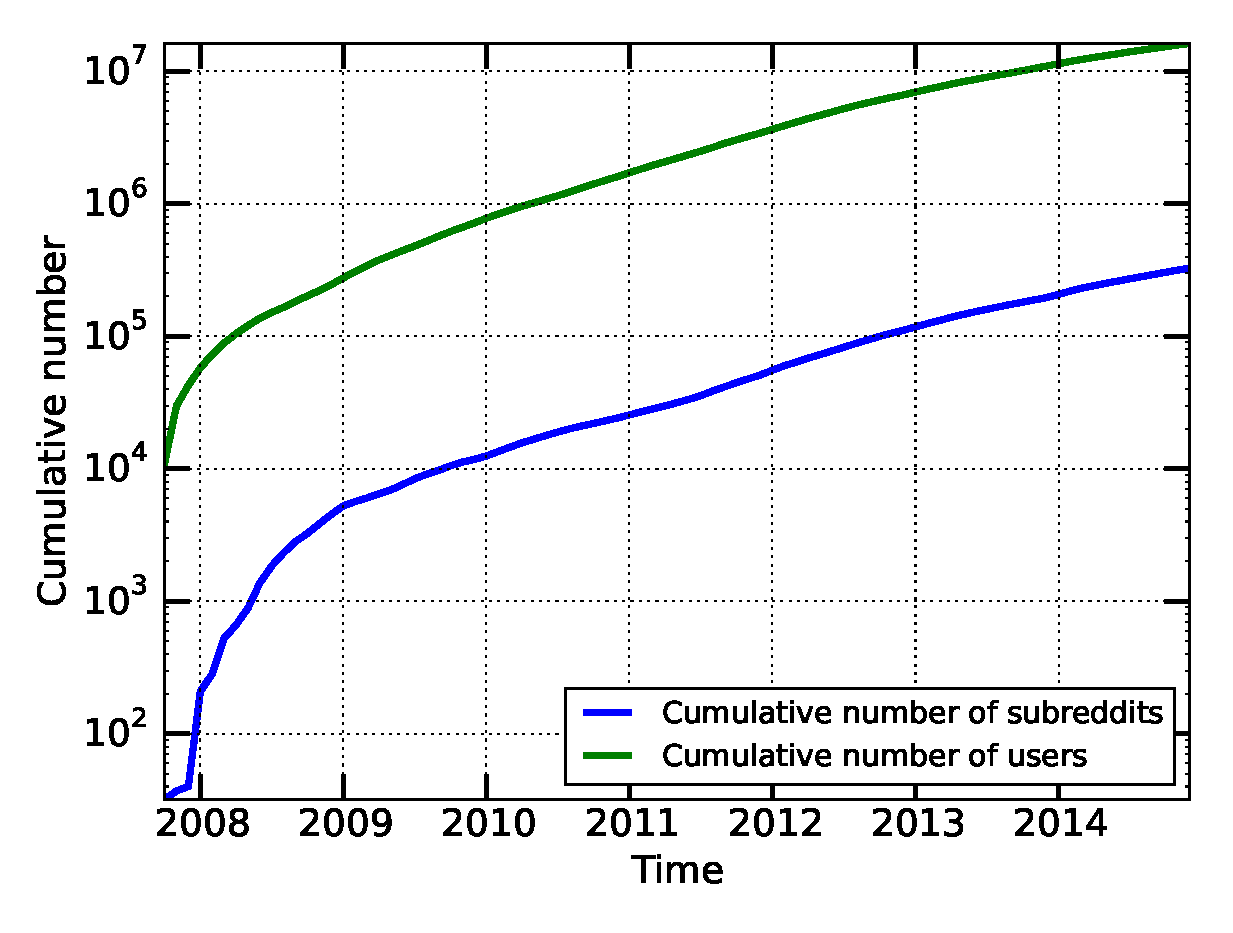
\includegraphics[scale=0.4]{./images/cumulative_users_subreddits.eps}
\caption{Caption}
\label{fig:cumulative_users_subreddits}
\end{figure}

We have identified that about 16.2 million distinct registered users made comments in reddit since its conception until the end of 2014, while around 327 thousand subreddits received comments. 

Since not all users post every month, the cumulative value might not be representative of how many users actually use reddit. If we consider only the users that authored a comment and the subreddits that had comments written at, we have the following graph.

\begin{figure}[!tb]
\centering
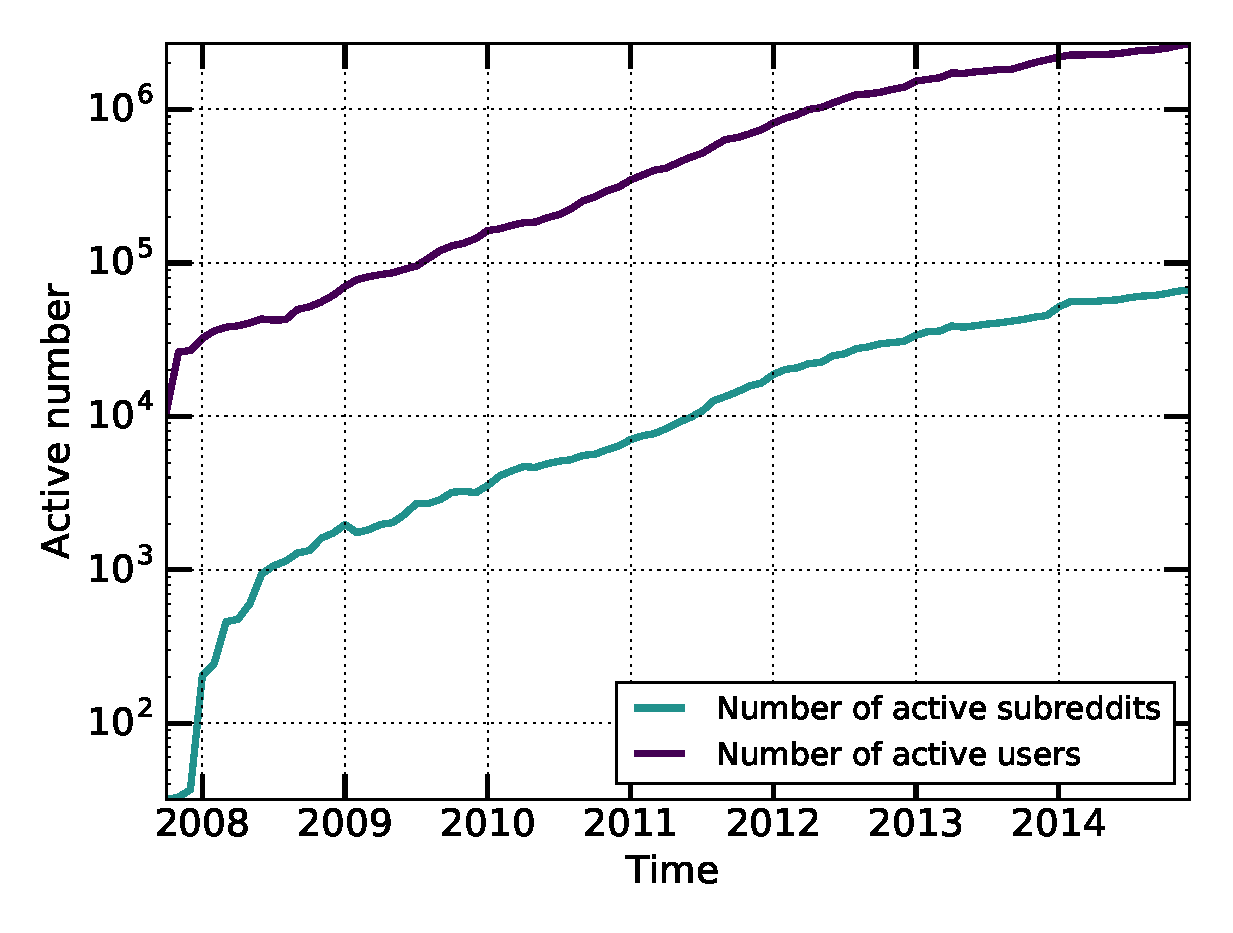
\includegraphics[scale=0.4]{./images/active_users_subreddits.eps}
\caption{Caption}
\label{fig:active_users_subreddits}
\end{figure}

In this graph, we can see that reddit had around 470 thousand users that made comments in the last month of 2014, while around 11400 subreddits received comments in this same month. While the cumulative growth of reddit is impressive, the actual active community is significantly smaller than the total number of existing registered users and subreddits, as expected.

The fact that such a significant amount of users stopped using the platform raises questions such as why users give up on their accounts, when they do so and which users are more likely to stay active. 

\subsection{Identifying cohorts}
%% Amit 9: Added this subsection here. Having the cohorts defined as the part of the overview will help, as we talk about them throughout the paper. Some of the cohort stuff from next section can come here. 